\documentclass[10pt,preprint]{sigplanconf}

%\ConferenceName{ACM ONWARD Papers 2015}
%\ConferenceShortName{ONWARD 2015}

%\usepackage{fullpage}
\usepackage{natbib}
\usepackage{breakurl}
\usepackage{algorithmic}
\usepackage{alltt}
\usepackage[ruled]{algorithm2e}
\usepackage[cmex10]{amsmath}
\usepackage{url} 
\usepackage{graphicx}
\usepackage{listings}
\usepackage{wrapfig}
\usepackage{multirow}
%\usepackage[plainpages=false, colorlinks=true, urlcolor={cyan}, citecolor={red}, linkcolor={green}]{hyperref}
\usepackage[plainpages=false]{hyperref}
\usepackage{array}
\usepackage{balance}
\usepackage{subfigure}
\usepackage{amssymb}
\usepackage{float}
\usepackage{caption}
\usepackage{placeins}
\usepackage{harmony}

% % % % % % % % % % % % % % % % % % % % % % % % % % % % % % % % 
\lstset{frame=none, xleftmargin=15pt, stepnumber=1, numbers=left, numbersep=5pt,
numberstyle=\tiny, belowcaptionskip=\bigskipamount,
captionpos=b, escapeinside={*'}{'*}, language=java, tabsize=2, emphstyle={\bf},
commentstyle=\it, stringstyle=\mdseries\ttfamily, showspaces=false,
keywordstyle=\bfseries, morekeywords={in,do,print,Metadata,Where}, columns=flexible,
basicstyle=\footnotesize\ttfamily, showstringspaces=false, morecomment=[l], mathescape=true}



\newcommand{\solution}{\bigskip\hrule\bigskip}
\newcommand{\problembreak}{\bigskip\hrule\bigskip}

\renewcommand{\theenumi}{\bf\Alph{enumi}}

\newlength{\spread}
\setlength{\spread}{1.0in}

\def\bibfont{\footnotesize}

% correct bad hyphenation here
%\hyphenation{op-tical net-works semi-conduc-tor}


%%%%%%%%%%%%%%%%%%%%%%% END of LaTeX definitions %%%%%%%%%%%%%%%%%%%%%%%%%%%%

\begin{document}

\permissiontopublish
\conferenceinfo{ONWARD~'15}{October 25--30, 2015, Pittsburgh, Pennsylvania, USA} 
\copyrightyear{2015} 
\copyrightdata{978-1-4503-1995-9/13/10} 
\doi{2508075.2514879} 

\title{An Objective Assessment of Musical Complexity: Translating Music Pedagogy's Deep Insights with Novel Computing Paradigms}

\authorinfo{Ethan Holder}
					 {Software Innovations Lab at Virginia Tech}
					 {eholder0@vt.edu}
					 
\authorinfo{Eli Tilevich}
					 {Software Innovations Lab at Virginia Tech}
					 {tilevich@cs.vt.edu}
					 
\authorinfo{Amy Gillick}
					 {Department of Music at Virginia Tech}
					 {agillick@vt.edu}
					 
%\authorinfo{R. Ben Knapp}
%					 {Center for the Arts at Virginia Tech}
%					 {benknapp@vt.edu}

\maketitle



\begin{abstract}

In the Western classical tradition, musicians play music from notated sheet music, called a score. When playing music from a score, a musician translates its visual symbols into sequences of instrument-specific physical motions. Hence, a music score's overall complexity represents a sum of the cognitive and mechanical acuity required for its performance.

At the technical level, this interdisciplinary research exploits a fundamental musical tenet that for a given instrument, different notes, intervals, and key signatures represent dissimilar levels of difficulty, which vary depending on the performer's proficiency. Tempo, dynamics, and articulation also affect the overall difficulty. We have realized our approach as a two-phase process. First, music experts rank the relative difficulty of musical components for different playing proficiencies and instruments. Second, an automated algorithm applies this ranking to music scores and calculates their respective complexity. Once music experts agree upon the complexity ranking for a given level of proficiency, our approach automatically calculates a music score's relative difficulty. The results of this interdisciplinary research project will empower musicians to expeditiously assess a music score's suitability for the abilities of intended performers.

This project is the first attempt to create a systematic and objective approach to assessing the complexity of a music score. The approach leverages computing technologies to be able to automatically and accurately calculate the complexity of playing a music score on a given instrument. As a proof-of-concept of the approach, we have been developing an automated, Web-based application for music educators and performers. This interdisciplinary research creates novel computing paradigms that systematically translate deep insights of Music Pedagogy, benefiting a broad music audience. Although the end product of this research will largely benefit musicians, the created novel computing concepts and paradigms will enhance the state of the art in computing, being applicable to solving important problems in other domains.

\end{abstract}

%\category{D.2.2}{Software Engineering}{Design Tools and Techniques}[Evolutionary prototyping \and Computer-aided software engineering (CASE)]
\keywords{Software; Software Engineering; Music; Translation; Assessment; Scoring; MusicXML; Java; Javascript


\section{Introduction} 
\label{sec:intro}

Below, we formally introduce this project by addressing its motivation \ref{sec:motiv} and outlining its associated research questions and goals \ref{sec:rqg} before laying out the remainder of this paper \ref{sec:layout}.

\subsection{Motivation} 
\label{sec:motiv}

Musicians often debate and disagree about the relative complexity of music scores, while the ability to accurately assess a score's complexity is required for curricular recommendations, competition specifications, etc. Additionally, people buying sheet music face great uncertainty when determining whether unfamiliar music matches their playing ability. Unfortunately, determining the relative complexity of music is a non-trivial cognitive task. Additionally, methods in the current state of the art depend solely on individual opinions, a process influenced by personal biases and lacking common criteria. By combining expertise from the fields of Computer Science and Music Pedagogy, this project aims to finally offer an objective solution to these debates.

While this work may seem like it addresses an unorthodox software engineering problem, in fact determining the relative complexity of music has many analogues in software. Consider figure \ref{image:complexities} which shows the different types of complexity associated with playing music. It also shows one typical scenario for generating output from high-level code. In both the cognitive tasks of interpreting high-level code and reading music notes, relatively short, expressive statements are transformed into complex actions to be performed. Then both take those actions and perform them to generate some kind of output. 

\begin{figure}[ht!]
	\centering
		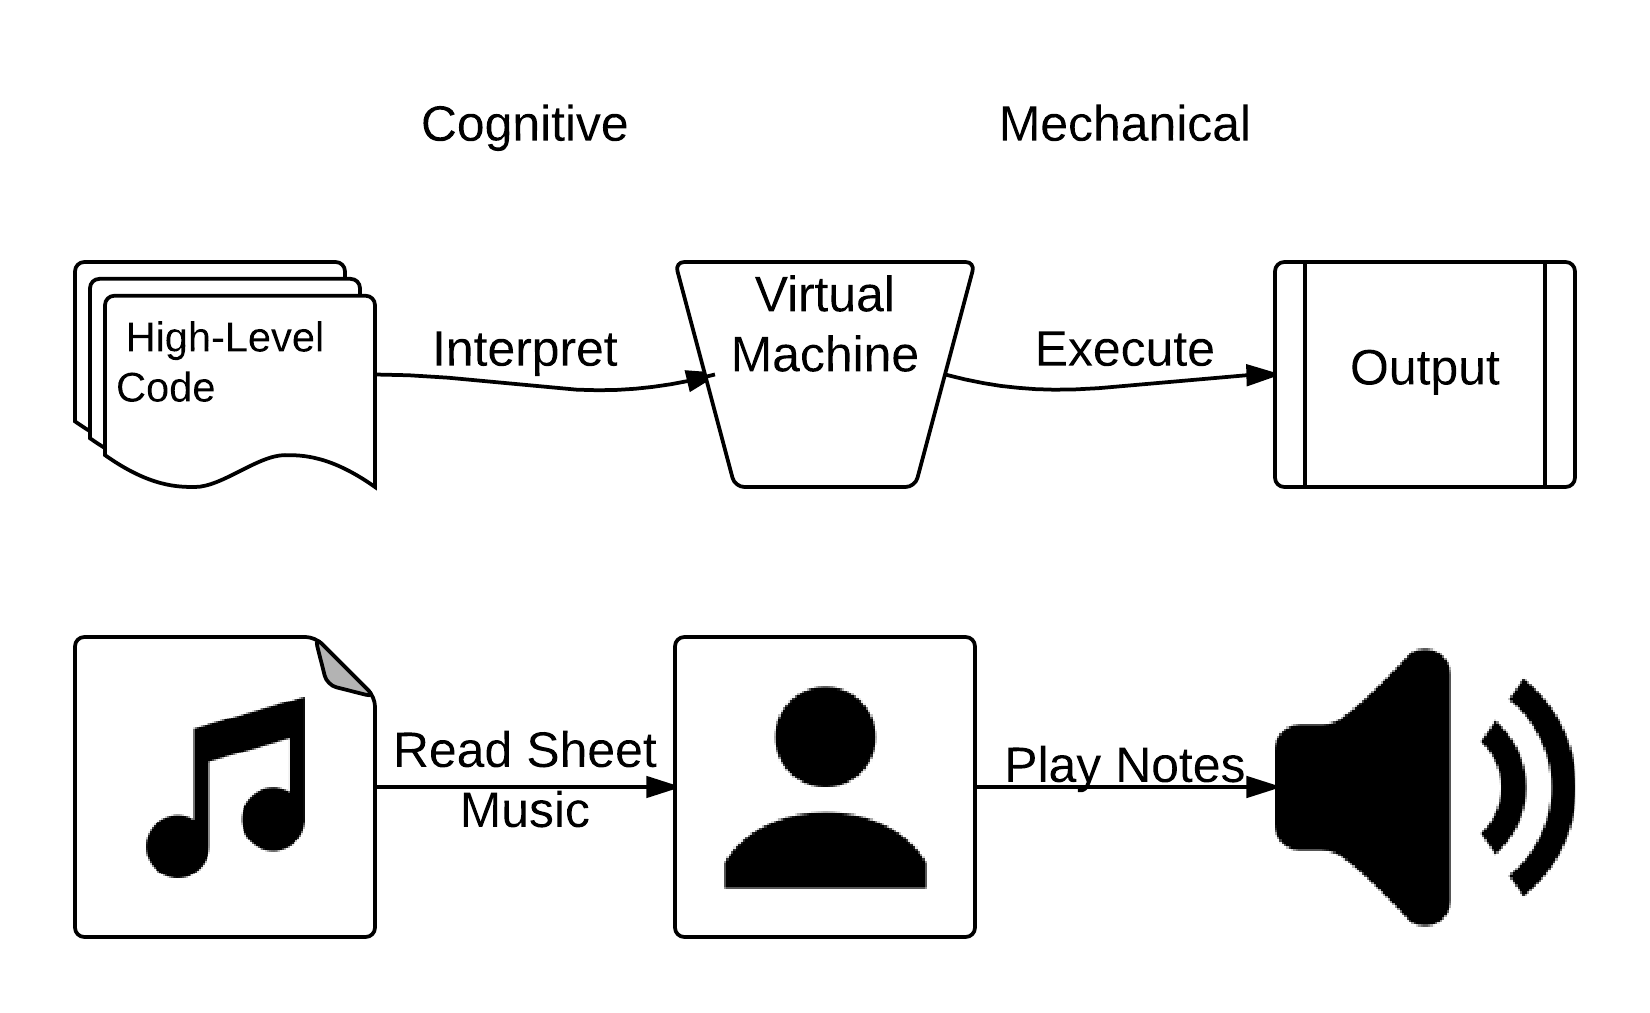
\includegraphics[width=0.47\textwidth]{CognitiveMechanical.png}
		\caption{The process of playing music introduces cognitive and mechanical complexities in reading and playing notes, respectively, just like interpreting high-level code into a virtual machine and executing it to produce output.}
		\label{image:complexities}
\end{figure} 

There are many other analogies to be drawn between music and software, but this one clearly shows how intricate a problem it can be to determine the complexity of music. Just as virtual machines uniformly interpret high-level code across physical machines (within one given language set), the execution of this interpreted form can vary wildly across different underlying architectures. The same is true of music. All musicians can read one piece of sheet music and understand it similarly, but the mechanical operation of playing that music on different instruments can represent many different complexities. This project hopes to blaze a trail towards addressing these complexities by creating a framework that can handle these subtle nuances.

%Move the motivating parts from the abstract down to here and make it flow together. This should flow naturally out of the background and abstract to present the general problem in the current state of the art.

\subsection{Research Goal \& Questions} 
\label{sec:rqg}

The overall goal of this paper is \textbf{to present a new approach to measuring the complexity of music pieces that is both objective and easy to use}. In doing so, we aim to answer the following research questions which have guided us throughout the project:

\begin{enumerate}
\item What musical elements should make up the complexity of musical pieces?
\item How should these elements factor into a complexity score?
\item How should each element be weighted on each instrument, specifically on B$\flat$ Clarinet?
\item What tools do musicians and educators need to access these complexity scores?
\item Are the current grades for competition pieces relatively correct?
\item What weights would be necessary to make those grades match complexity scores (if they can be made to do so)?
\end{enumerate}


\subsection{Paper Layout} 
\label{sec:layout}

The remainder of this paper is structured as follows. First, background information on music is presented to provide a base line for readers in section \ref{sec:background}. Then, related work in this field is highlighted in section \ref{sec:related}. Next, we explain the implementation of our scoring system in section \ref{sec:imple}. This leads into the experimental setup which shows the current difficulty settings in section \ref{sec:experiment}. The results in section \ref{sec:results} then show exactly what we have uncovered through the implementation and user experiments so far. The analysis section \ref{sec:analysis} follows after the results and discusses how our system compares to others in the wild. Next, brief directions for future work are given in section \ref{sec:future}. Finally, we present our conclusions for this project in section \ref{sec:conclu}.

\section{Background} 
\label{sec:background}

To better understand this research work as a whole, readers must first understand the basics of music. The following section will serve to enlighten readers about elements of sheet music covered in this work. \footnote{Portions of the background section are not exactly correct. That is, they represent a simplified view of music theory that abstracts away many concepts for the benefit of readers with no prior experience and for brevity.}

The fundamental building block of music is the note. Notes in music are similar to words in spoken language or characters in code. Notes have several characteristics and can thus take many forms. The most important characteristics of notes in written music are pitch, duration, dynamics, and articulation. On sheet music, notes are represented with different ovals both with and without a line - or stem - attached to it. Notes are placed into measures. A measure is a uniform amount of time that breaks up a song into smaller portions and is somewhat analogous to a sentence in spoken language.

Pitch is the most obvious characteristic of any note. It is the frequency of the sound wave the note produces. It is how high or low a note sounds to the listener. Pitches are not continuous, but rather fall on specific discrete steps or half steps within the range of audible frequencies. Intervals are the difference in pitches between two or more notes. There are several names for intervals based on how far apart the pitches are and whether the difference falls on a full or half step.

The pitch of a note can be determined from the note's vertical placement on the staff (the five horizontal lines and four spaces between), the clef (the range of notes possible to represent on the staff), and the key signature (the notes whose pitch should be altered up or down a half step). Accidentals can also similarly alter the pitch of a note up or down a half step, but accidentals are not applied to the entire song, only one specific note at a time. Both accidentals and the key signature are represented by symbols called sharps or $\sharp$, which raise the pitch a half step, flats or $\flat$, which lower the pitch a half step, and naturals or $\natural$, which returns the pitch of a previously altered note back to its normal pitch.

Duration is simply how long a note is played or held out. Duration is not directly specified in written music, but it can be determined through the note's value (a fraction relative to whole which can be seen by the stem and flag attached to a note), the time signature (how many beats are in a measure and what fraction of a whole note gets a beat), and the tempo (how my beats are played in a given time frame).

For example, a quarter note receives $1/4$th the beats of a whole note. In three four time, the first number says there are three beats in a measure, and the second number says that a quarter note receives one beat in a measure. In this example there would be 3 total beats in any measure. If the tempo is 120 bpm (beats per minute), then this example measure would last exactly 1.5 seconds (3 beats / (120 bpm / 60 seconds/minute)).

Dynamics refers to the overall loudness or volume of a note. Dynamics are specified with different Italian words, such piano (meaning soft), forte (meaning loud), and mezzo (meaning medium). Combining and stacking these leads to many possible dynamic levels, typically ranging from ppp (pianississimo, meaning very very soft) to fff (fortississimo, meaning very very loud). There are also markings for gradually changing dynamics to louder (crescendo) or softer (decrescendo or alternatively diminuendo) that look like elongated greater than or less than symbols below the staff.

Articulation is how a note is played and linked to subsequent notes. The simplest analogy for articulations are how different letters or sounds are formed and connected in spoken language. For example, speaking "ta" and "la" have the same sound once held out, but their initial articulations are different based on how people make the "t" and "l" sounds. There are many different articulations, but the main ones utilized in this work are as follows:

\begin{itemize}
\item Accent or $>$, which means to play the note louder than those around it.
\item Staccato or $\cdot$, which means to play the note shorter than its full value, cutting it off early.
\item Tenuto or -, which means to play the note slightly longer than its full value, barely cutting it off before the next note.
\item Marcato (or strong accent) or $\wedge$, which means to play the note much louder than those around it, more than an accent.
\item Slur or $\smile$, which means not to separate all notes after the first but to connect them together.
\end{itemize}

There are more characteristics of notes, such as timbre, but for the purposes of this project, they have been ignored. Composers combine all of the concepts above and more when writing music. No one is more important than another, but understanding this subset at least is essential to this research work.

%Provide an overview of music concepts, what they mean, how they impact play, and generally define our terms for the remainder of the paper. This could also probably stand alone after the abstract as its own section depending on its size. We'll need to be careful not to let this cover too much space even though we'll need to cover a lot of information.

\section{Related Work} 
\label{sec:related}

Cover any related work in the field and differentiate this project.

\section{Implementation} 
\label{sec:imple}

The first subsection below will explain how to form the complexity score from the concepts above in \ref{sec:scoring}.  Next, we go into the basic approach to this project and how it naturally extends itself in \ref{sec:design}. Finally, we cover the low level details of how this is accomplished in \ref{sec:details}.

\subsection{Complexity Score} 
\label{sec:scoring}

In the background section above \ref{sec:background}, many fundamental music concepts were discussed. Those concepts serve as the baseline elements that factor into the complexity score. The initial idea for this project was as follows: arbitrarily assign weights to each of those concepts or elements from above, determine when and how often each occurs in the piece of music, and finally add up the weights for each occurrence before outputting it to the user.

%I need to explain what concepts we actually use and how they're combined here...

We initially experimented with giving whole number weights to each element we perceived to be especially important (ie notes, intervals, dynamics, articulations, key signatures, and note durations). This worked, but it did not seem exactly analogous to our experiences with playing music. At their core, notes and intervals seemed to present distinct difficulties on their own, whereas dynamics, articulations, key signatures, and note durations seemed to modify those difficulties. For instance, a small interval may seem easy on its own, but with changing dynamics, with differing articulations, in a strange key, or at a high speed, that interval could become much more difficult.

From there, we modified our approach so that only notes and intervals received weights as whole numbers. These were still counted and summed up for a total score. However, dynamics, articulations, key signatures, and note durations became multipliers onto notes and intervals. Each dynamic, articulation, and key signature thus receives a multiplier weight that is a decimal (typically between 0 and 2). Those multipliers are applied to every occurrence of a note and interval.

Note duration is factored into the score as an average over all notes. The total amount of notes and associated duration in seconds is calculated at the end and applied as its own multiplier. The more notes in a given span of time, the higher the multiplier becomes.

This seems to capture the concept we envisioned that makes duration complex, except in the case of playing extremely long notes. In such cases on wind instruments, holding notes out for significantly long amounts of time possess its own difficulty in providing the breath support rather than quickly moving fingers.

Thus, we adapted the note duration measurement to be a multiplicative difference from one. Therefore, if the average of notes per second in the piece was 1.5, then the multiplier remained 1.5. However, in the case of many long notes, the average of notes per second might be something closer to 0.5. In this case (when the average is less than 1) the multiplier becomes its reciprocal, 2 in this case. Users cannot directly change this parameter, however they can provide a multiplier value for note duration that is multiplied to the result of this calculation before it is applied to the total score. By default this parameter is set to 1.

\subsection{Design Overview} 
\label{sec:design}

Our approach to determining a complexity score has served us well so far, but the full control flow of this project involves many more steps. A diagram of the overall process can be seen in figure \ref{image:flow}.

\begin{figure}[ht!]
	\centering
		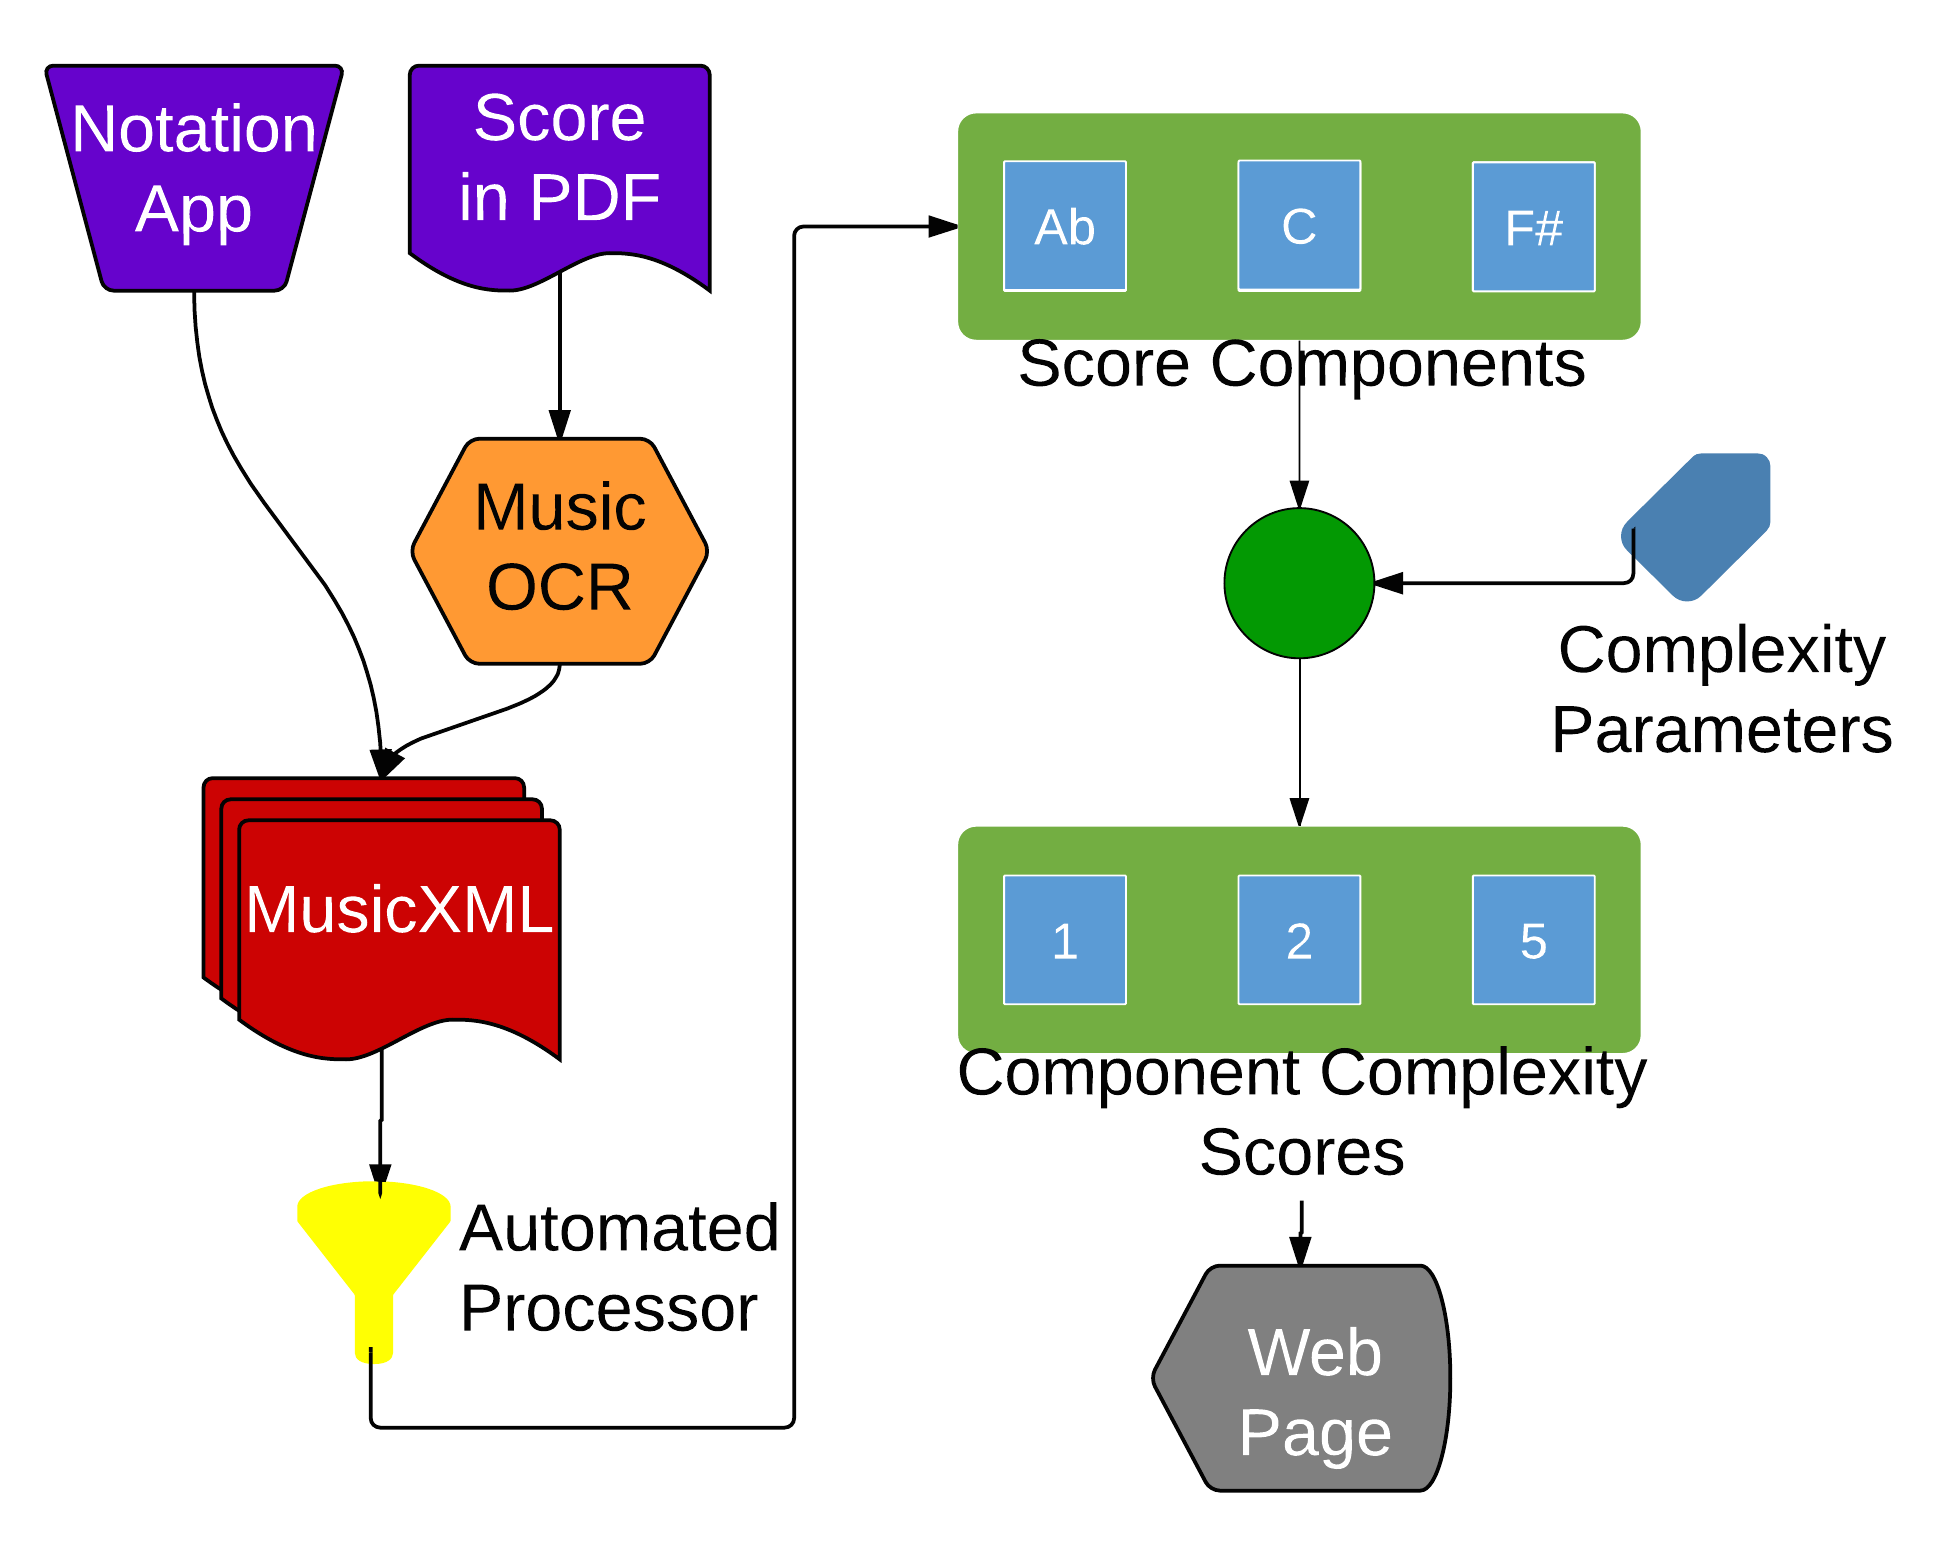
\includegraphics[width=0.47\textwidth]{JoinedCropped.png}
		\caption{The overall control flow from a user's perspective.}
		\label{image:flow}
\end{figure}

From the top left, we see that the inputs to this project are Notation Apps and Scores in PDF format \footnote{Score here means a musical score or piece of music, not a complexity score.}. Many common notation applications, such as Finale Notepad \cite{FinaleNotepad} and Sibelius \cite{Sibelius}, support a universal format called MusicXML \cite{MusicXML}. MusicXML files can be imported into those applications, edited, and output back to MusicXML or other proprietary formats. MusicXML is the underlying representation that this project operates on.

Alternatively, we have support for music pieces in PDF format. We can accept PDF files and transform them into their MusicXML representation using music OCR (Optical Character Recognition) software. Our reference implementation relies on free software from Audiveris \cite{Audiveris} currently, but it could equivalently utilize other off the shelf products.

Once we have the MusicXML representation of the piece, it is passed into the automated processor. The processor then perform the essential steps from above. It pulls specific components out of the piece as it parses through. It then looks up the weights for each component as specified by the complexity parameters. These parameters can be easily changed through creating a new xml file to specify them. We provide 5 different default files, ranging from a beginner's level of play up to a trained professional's level of play.

Using the specified weights, we can then perform several calculations on the piece, such as determining the overall complexity score, separating the score out by notes or by intervals, and finding the most complex measure and its score. The results of each of these calculations are finally formatted and passed up to the calling web page that presents the UI \footnote{The current version can be found at \url{http://mickey.cs.vt.edu/}}.

The key with this approach is that it is easily extensible at each level. Any platform that can generate MusicXML can feasibly serve as an input to our program. Furthermore, the overall process can be extended if other applications can generate the piece of music in PDF form or some intermediary that can be reduced down to PDF or MusicXML.

The algorithm itself can be extended to operate only on specific selections of pieces or on batches of multiple pieces if necessary (thus showing the complexity of an entire concert). Finally, the parameters that determine complexity can easily be changed on the fly. This allows individual performs or groups to set their own complexity levels to find a score even more relevant to their playing style.


%Talk about the high level approach for how this works in terms of the musical elements defined in the background section earlier.

\subsection{Code Details} 
\label{sec:details}

This project spans several different code bases, most notably the automated processor backend and the web UI frontend. The entire source code for this project is available for public consumption on GitHub \footnote{\url{https://github.com/xwsxethan/MusicScoring}} \cite{GithubMusicScoring} with instructions as to how to set it up and run it on one's own.

The backend code is written entirely in Java with some limited PHP to facilitate server communication. We've utilized the Apache Xerces 2.11.0 library for parsing xml files \cite{XMLAPI} and the JSON Simple 1.1.1 library for constructing JSON to pass along \cite{JSONAPI}. The backend utilizes the visitor pattern so as to easily handle the intricacies and redundancies of scanning MusicXML.

The frontend code is written in standard Javascript, HTML, and CSS. We utilize numerous libraries here for simplicity, including jQuery 2.1.0 \cite{jQuery}, Bootstrap 3.3.4 \cite{Bootstrap}, DataTables 1.10.5 \cite{DataTables}, D3 3.5.5 \cite{D3}, and VexFlow 1.2.27 \cite{VexFlow}. Each of these allows us to more easily present the underlying data and make it more accessible to end users.

%Very briefly talk about the actual implementation details. This should not span more than a paragraph or two just talking about the lines of code written, the libraries used, and the languages utilized.

\section{Experimental Setup} 
\label{sec:experiment}

In order to run any tests and compare our results, we first have to setup some basic complexity parameters. We specify the settings we've used and where they came from in \ref{sec:settings}. After, we unveil how we plan to adjust those settings in the future in \ref{sec:survey}.

%Describe the preliminary settings used to score pieces based on clarinet and how we plan to refine them. Also talk about usability

\subsection{Clarinet Complexity Settings} 
\label{sec:settings}

Section \ref{sec:scoring} above discusses where the form of complexity parameters came from and why. It shows which types of parameters became whole number weights and which became decimal number multipliers. These were presented in a general sense without being linked to a given instrument. This sections discusses their specific form for one such instrument, B$\flat$ clarinet.

We decided to focus on the clarinet specifically, because it exhibits many forms of complexity and represents many similar woodwind and brass instruments. Additionally, our own musical expertise lies more in that instrument above all others so we felt most qualified to define our own complexity parameters there.

The initial complexity settings for B$\flat$ Clarinet were for beginners. Based on these values, complexity settings for other levels of B$\flat$ Clarinet were later adapted, but largely changed only associated weights. Note complexities were broken up into the ranges (inclusive) and assigned weights shown in table \ref{table:notes}. Intervals were similarly broken up further and assigned weights as shown in table \ref{table:intervals}.  

\begin{table}[t]
	\centering
    \begin{tabular}{| l | l |}
        \hline
        Note Range & Weight \\ \hline
        G3-G$\sharp$4 & 1 \\ \hline
        A4 & 2 \\ \hline
        B$\flat$4-C5 & 5 \\ \hline
        $\geq$ C$\sharp$5 & 10 \\
        \hline
    \end{tabular}
	\caption{The note ranges and weights for beginner B$\flat$ Clarinet.}
	\label{table:notes}
\end{table}

\begin{table}[t]
	\centering
    \begin{tabular}{| l | l | l | l |}
        \hline
        Interval & Low Range & High Range & Weight \\ \hline
        Unison & Anywhere & Anywhere & 1 \\ \hline
        Second & G3-G$\sharp$4 & G3-G$\sharp$4 & 2 \\ \hline
        Third & G3-G$\sharp$4 & G3-G$\sharp$4 & 3 \\ \hline
        Fourth & G3-G$\sharp$4 & G3-G$\sharp$4 & 4 \\ \hline
        Fifth & G3-G$\sharp$4 & G3-G$\sharp$4 & 5 \\ \hline
        Any & G3-G$\sharp$4 & A4-C5 & 8 \\ \hline
        Any & A4-C5 & $\geq$ C$\sharp$5 & 10 \\ \hline
        Sixth & Anywhere & Anywhere & 9 \\ \hline
        Seventh & Anywhere & Anywhere & 9 \\ \hline
        Octave & Anywhere & Anywhere & 9 \\ \hline
        $>$ Octave & Anywhere & Anywhere & 10 \\
        \hline
    \end{tabular}
	\caption{The intervals, note ranges, and weights for beginner B$\flat$ Clarinet.}
	\label{table:intervals}
\end{table}

Dynamics and articulations were specified for those specific types mentioned previously in section \ref{sec:background}. Their weights can be found in tables \ref{table:dynamics} and \ref{table:articulations}, respectively. Unlike dynamics and articulations, all possible major key signatures are specified with weights and shown in table \ref{table:key}. Finally, the note duration modifier is kept at 1.0, so the note duration modifier works exactly as specified in \ref{sec:scoring}.

\begin{table}[]
	\centering
    \begin{tabular}{| l | l | l |}
        \hline
        Dynamic & Abbreviation & Weight \\ \hline
        mezzo forte & mf & 1.0 \\ \hline
        mezzo piano & mp & 1.0 \\ \hline
        forte & f & 1.1 \\ \hline
        fortissimo & ff & 1.2 \\ \hline
        piano & p & 1.3 \\ \hline
        pianissimo & pp & 1.5 \\
        \hline
    \end{tabular}
	\caption{The dynamics and weights for beginner B$\flat$ Clarinet.}
	\label{table:dynamics}
\end{table}

\begin{table}[]
	\centering
    \begin{tabular}{| l | l |}
        \hline
        Articulation & Weight \\ \hline
        Slur & 0.5 \\ \hline
        Normal/None & 1.0 \\ \hline
        Accent & 1.1 \\ \hline
        Staccato & 1.2 \\ \hline
        Tenuto & 1.2 \\ \hline
        Marcato (Strong Accent) & 1.4 \\
        \hline
    \end{tabular}
	\caption{The articulations and weights for beginner B$\flat$ Clarinet.}
	\label{table:articulations}
\end{table}

\begin{table}[]
	\centering
    \begin{tabular}{| l | l | l |}
        \hline
        Key Signature & Sharps/Flats & Weight \\ \hline
        C & None & 1.0 \\ \hline
        G & F$\sharp$ & 1.1 \\ \hline 
        D & F$\sharp$, C$\sharp$ & 1.1 \\ \hline
        A & F$\sharp$, C$\sharp$, G$\sharp$ & 1.2 \\ \hline
        E & F$\sharp$, C$\sharp$, G$\sharp$, D$\sharp$ & 1.3 \\ \hline
        B & F$\sharp$, C$\sharp$, G$\sharp$, D$\sharp$, A$\sharp$ & 1.4 \\ \hline
        F$\sharp$ & F$\sharp$, C$\sharp$, G$\sharp$, D$\sharp$, A$\sharp$, E$\sharp$ & 1.5 \\ \hline
        C$\sharp$ & F$\sharp$, C$\sharp$, G$\sharp$, D$\sharp$, A$\sharp$, E$\sharp$, B$\sharp$ & 1.6 \\ \hline
        F & B$\flat$ & 1.1 \\ \hline
        B$\flat$ & B$\flat$, E$\flat$ & 1.1 \\ \hline
        E$\flat$ & B$\flat$, E$\flat$, A$\flat$ & 1.2 \\ \hline
        A$\flat$ & B$\flat$, E$\flat$, A$\flat$, D$\flat$ & 1.3 \\ \hline
        D$\flat$ & B$\flat$, E$\flat$, A$\flat$, D$\flat$, G$\flat$ & 1.4 \\ \hline
        G$\flat$ & B$\flat$, E$\flat$, A$\flat$, D$\flat$, G$\flat$, C$\flat$ & 1.5 \\ \hline
        C$\flat$ & B$\flat$, E$\flat$, A$\flat$, D$\flat$, G$\flat$, C$\flat$, F$\flat$ & 1.6 \\
        \hline
    \end{tabular}
	\caption{The major key signatures and weights for beginner B$\flat$ Clarinet.}
	\label{table:key}
\end{table}



\subsection{External Survey} 
\label{sec:survey}

Although the complexity settings presented in \ref{sec:settings} may in fact be accurate, there is no means of validating them empirically. They are simply best guesses based on personal experiences. Moreover, there is no way to empirically validate the ``correctness'' of an overall score since there is no standard for the complexity of a piece. However, if there can be a general agreement from those with a stake in the score, then that may be validation enough.

Based on this assumption, experts, musicians, and educators seem to have a vested stake in the results of these complexity scores. Therefore, we've begun to survey those related to B$\flat$ Clarinet in an effort to ascertain their opinions. In the survey we ask simple questions about the complexity parameters already established, both how the parameters are implemented and the weights assigned to each. Once a statistically significant consensus has been reached or some threshold of responses have been given, the results of the survey will become the new complexity parameters. At the time of writing, neither condition has been met so our own parameters are in use, but it is important to note that we are striving to find an amicable means of setting these parameters.

\section{Results} 
\label{sec:results}

Talk about our scores for various pieces and graph the results. We can talk about how it works for multiple parts, but we have to mention that the current settings are not meant for different instruments. Also cover any results we may have from the survey at that time (if any).

The table \ref{table:difference} shows data about Audiveris using the beginner score settings.

\begin{table}[ht!]
	\centering
    \begin{tabular}{| l | l | l | l | l |}
        \hline
        Type & Words & Lines & Char's & Score \\ \hline
        Original & 20964 & 27451 & 580569 & 215546 \\ \hline
        Converted & 21584 & 30825 & 783894 & 298655 \\ \hline
        Difference & 10202 & 38200 & 736456 & 83109 \\ \hline
        Normalized & 0.4866 & 1.3916 & 1.2685 & 0.3856 \\
        \hline
    \end{tabular}
	\caption{The words, lines, and characters of the original MusicXML, the OCR converted MusicXML, the difference between them, and the normalized difference based on the original.}
	\label{table:difference}
\end{table}

\subsection{Usability} 
\label{sec:usability}

Talk about how the website is setup to be very user friendly and easy to navigate. 

\section{Analysis} 
\label{sec:analysis}

Compare our results from objectively scoring to similar scoring methods by state school groups. Talk about the opportunities for this methodology to expand as well as its usefulness.

\section{Future Work} 
\label{sec:future}

Talk about the challenges we haven't addressed but want to next, like scaling the score range to between 1 and 100, joining this technology with International Music Score Library Project \footnote{\url{http://imslp.org/}}, leveraging SeeMore to show it off, and associating different part names to various instruments.

Outline plans to survey more people and expand difficulties for parts.

Also talk about the point Jason raised in the reading group: reverse engineer this setup and use some creative linear algebra to determine what parameters would be necessary in order for the rankings of state repertoire pieces to match up correctly. As in, given some 1-5 rankings, determine what difficulty settings we need for this method to output complexity scores that fit within 1-5 multiplied by some $\alpha$ that scales the values up and within some range $\beta$ that gives a plus or minus from the scaled values. Tighten up $\beta$ as much as possible.

\section{Conclusions} 
\label{sec:conclu}

Sum up the paper.

\section*{Acknowledgments} 
\label{sec:ack}

Thank everyone and list any outside funding or support.




% The bibliography should be embedded for final submission.
\medskip
%\nocite{*}
%\bibliographystyle{abbrvnat}
\bibliography{HolderOnward2015}
\bibliographystyle{abbrv}


\end{document}